\begin{table}[H]
	\centering
	\sffamily\scriptsize
	\setlength{\tabcolsep}{4pt}
	\renewcommand{\arraystretch}{1.3}
	\caption{Ficha técnica --- UTM SonicWall NSa 6600}\label{table:utm}
	\begin{tabular}{|p{0.25\textwidth}|p{0.6\textwidth}|p{0.12\textwidth}|}
		\hline
		\rowcolor{gray!15} \multicolumn{3}{|c|}{\textbf{DESCRIPCIÓN FÍSICA:} Dispositivo de seguridad perimetral (UTM)} \\ \hline

		\textbf{TIPO DE RECURSO:} & Firewall / UTM &
		\multirow{3}{*}{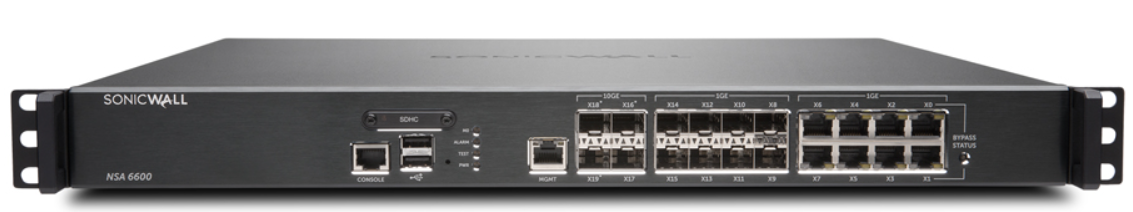
\includegraphics[width=\linewidth,keepaspectratio]{tablas-images/utm/utm.png}} \\ \cline{1-2}
		\textbf{MODELO:} & NSa 6600 & \\ \cline{1-2}
		\textbf{MARCA:} & SonicWall & \\ \hline

		\rowcolor{gray!15} \multicolumn{3}{|c|}{\textbf{FUNCIONALIDADES DE SEGURIDAD}} \\ \hline

		\textbf{Firewall} &
		\begin{minipage}[t]{\linewidth}
			\vspace{2pt}
			• Inspección profunda de paquetes (DPI) \\
			• Control de acceso basado en políticas \\
			• Prevención de ataques DoS/DDoS
			\vspace{2pt}
		\end{minipage} & \\ \hline

		\textbf{IDS/IPS} &
		\begin{minipage}[t]{\linewidth}
			\vspace{2pt}
			• Sistema de prevención de intrusiones integrado \\
			• Detección de tráfico malicioso en tiempo real
			\vspace{2pt}
		\end{minipage} & \\ \hline

		\textbf{VPN} &
		\begin{minipage}[t]{\linewidth}
			\vspace{2pt}
			• VPN IPSec y SSL \\
			• Soporte para múltiples túneles site-to-site y acceso remoto
			\vspace{2pt}
		\end{minipage} & \\ \hline

		\textbf{Filtrado y control} &
		\begin{minipage}[t]{\linewidth}
			\vspace{2pt}
			• Filtrado web basado en reputación \\
			• Control de aplicaciones \\
			• Protección antimalware
			\vspace{2pt}
		\end{minipage} & \\ \hline

		\rowcolor{gray!15} \multicolumn{3}{|c|}{\textbf{ESPECIFICACIONES TÉCNICAS}} \\ \hline

		\textbf{Throughput Firewall} & 12 Gbps & \\ \hline
		\textbf{Throughput DPI} & 3.0 Gbps & \\ \hline
		\textbf{Throughput IPS} & 4.5 Gbps & \\ \hline
		\textbf{Throughput VPN} & 5.0 Gbps & \\ \hline
		\textbf{Conexiones simultáneas (SPI)} & 1,500,000 & \\ \hline
		\textbf{Nuevas conexiones/seg} & 90,000/sec & \\ \hline

		\rowcolor{gray!15} \multicolumn{3}{|c|}{\textbf{CAPACIDADES DE RED}} \\ \hline

		\textbf{Interfaces} & Puertos Ethernet 1GbE/10GbE según configuración & \\ \hline
		\textbf{VPN Site-to-Site} & Hasta 6,000 túneles & \\ \hline
		\textbf{Clientes VPN} & Hasta 6,000 usuarios & \\ \hline
		\textbf{Protocolos} & BGP, OSPF, RIP v1/v2, VLAN, NAT & \\ \hline

		\rowcolor{gray!15} \multicolumn{3}{|c|}{\textbf{CARACTERÍSTICAS FÍSICAS}} \\ \hline

		\textbf{Alimentación} &  Fuente redundante AC & \\ \hline
		\textbf{Montaje} & Rack (entorno empresarial) & \\ \hline

		\rowcolor{gray!15} \multicolumn{3}{|l|}{\textbf{PROPÓSITO:} Protección perimetral de la infraestructura del \GRID mediante inspección, control y monitoreo del tráfico de red} \\ \hline
		\rowcolor{gray!15} \multicolumn{3}{|l|}{\textbf{OPORTUNIDAD DE USO:} Seguridad en entornos de computación en la nube del \GRID} \\ \hline

		\multicolumn{3}{|p{0.97\textwidth}|}{
		\textbf{OBSERVACIONES:} Dispositivo central en la arquitectura de seguridad, permite implementar estrategias de defensa en profundidad e integración con soluciones SIEM (Wazuh) e IDS/IPS (Suricata).
		} \\ \hline

	\end{tabular}
\end{table}